% \begin{filecontents*}{example.eps}
% %!PS-Adobe-3.0 EPSF-3.0
% %%BoundingBox: 19 19 221 221
% %%CreationDate: Mon Sep 29 1997
% %%Creator: programmed by hand (JK)
% %%EndComments
% gsave
% newpath
%   20 20 moveto
%   20 220 lineto
%   220 220 lineto
%   220 20 lineto
% closepath
% 2 setlinewidth
% gsave
%   .4 setgray fill
% grestore
% stroke
% grestore
% \end{filecontents*}
% %
% \RequirePackage{fix-cm}
% %
% %\documentclass{svjour3}                     % onecolumn (standard format)
% \documentclass[smallcondensed]{svjour3}     % onecolumn (ditto)
%\documentclass[smallextended]{svjour3}       % onecolumn (second format)
%\documentclass[twocolumn]{svjour3}          % twocolumn
%
%% as per the requirement new theorem styles can be included as shown below
%\theoremstyle{thmstyleone}%
%\newtheorem{theorem}{Theorem}%  meant for continuous numbers
%%\newtheorem{theorem}{Theorem}[section]% meant for sectionwise numbers
%% optional argument [theorem] produces theorem numbering sequence instead of independent numbers for Proposition
% \newtheorem{proposition}[theorem]{Proposition}% 
% %%\newtheorem{proposition}{Proposition}% to get separate numbers for theorem and proposition etc.

% \theoremstyle{thmstyletwo}%
% \newtheorem{example}{Example}%
% \newtheorem{remark}{Remark}%

% \theoremstyle{thmstylethree}%
%\newtheorem{definition}{Definition}%

%\raggedbottom
%%\unnumbered% uncomment this for unnumbered level heads
\documentclass[review]{elsarticle}

\usepackage[numbers]{natbib}
\usepackage{natbib}
\sloppy
\usepackage{graphicx}
\usepackage{multirow}
\usepackage{array}
\usepackage{caption, subcaption}
\usepackage{listings}
\usepackage{color}
\definecolor{codegreen}{rgb}{0,0.6,0}
\definecolor{codegray}{rgb}{0.5,0.5,0.5}
\definecolor{codepurple}{rgb}{0.58,0,0.82}
\definecolor{backcolour}{rgb}{0.95,0.95,0.92}
\lstdefinestyle{mystyle}{
	backgroundcolor=\color{backcolour},
	commentstyle=\color{codegreen},
	keywordstyle=\color{magenta},
	numberstyle=\tiny\color{codegray},
	stringstyle=\color{codepurple},
	numbers=left, numbersep=3pt}
\lstset{style=mystyle}
%\usepackage{geometry}
\usepackage{multirow}
\usepackage{booktabs}
\usepackage{rotating}

\newcolumntype{P}[2]{%
	>{\begin{turn}{#1}\begin{minipage}{#2}\small\raggedright\hspace{0pt}}l%
			<{\end{minipage}\end{turn}}%
}
%\usepackage{subfig}
%\newcolumntype{P}[1]{>{\centering\arraybackslash}p{#1}}
%
% \usepackage{mathptmx}      % use Times fonts if available on your TeX system
%
% insert here the call for the packages your document requires
%\usepackage{latexsym}
% etc.
%
% please place your own definitions here and don't use \def but
% \newcommand{}{}
%
% Insert the name of "your journal" with
% \journalname{myjournal}
%
\usepackage{lineno,hyperref}
\usepackage{breqn}
\usepackage{amsmath}
\usepackage{setspace}
\usepackage{multirow, multicol}
\usepackage{float}
\usepackage{algorithm}
\usepackage{algpseudocode}
\usepackage{xcolor}
%\usepackage{subfig}
\def\tsc#1{\csdef{#1}{\textsc{\lowercase{#1}}\xspace}}
\tsc{WGM}
\tsc{QE}
\tsc{EP}
\tsc{PMS}
\tsc{BEC}
\tsc{DE}
%%%
\journal{Information Processing and Management}

\begin{document}
\let\WriteBookmarks\relax
\def\floatpagepagefraction{1}
\def\textpagefraction{.001}
%\shorttitle{}

%
\begin{frontmatter}
\title{An Automated Hybrid Deep Model Approach Towards Sentiment Analysis for Online Product Reviews}
\author[label1]{Ashwin Perti}
\author[label2]{Amit Sinha}
\author[label3]{Ankit Vidyarthi}

\affiliation[label1]{organization={Department of Computer Science and Engineering, Galgotia University},%Department and Organization
            addressline={Plot No. 2, Sector 17A}, 
            city={Greater Noida},
            postcode={203201}, 
            state={Uttar Pradesh},
            country={India}}
\affiliation[label2]{organization={Department of Information Technology, ABES Engineering College},%Department and Organization
            addressline={NH-09}, 
            city={Ghaziabad},
            postcode={201009}, 
            state={Uttar Pradesh},
            country={India}}
\affiliation[label3]{organization={Department of Computer Science Engineering and Information Technology, Jaypee Institute of Information Technology Noida},%Department and Organization
	addressline={Sector-62}, 
	city={Noida},
	postcode={201309}, 
	state={Uttar Pradesh},
	country={India}}
%%=============================================================%%
%% Prefix	-> \pfx{Dr}
%% GivenName	-> \fnm{Joergen W.}
%% Particle	-> \spfx{van der} -> surname prefix
%% FamilyName	-> \sur{Ploeg}
%% Suffix	-> \sfx{IV}
%% NatureName	-> \tanm{Poet Laureate} -> Title after name
%% Degrees	-> \dgr{MSc, PhD}
%% \author*[1,2]{\pfx{Dr} \fnm{Joergen W.} \spfx{van der} \sur{Ploeg} \sfx{IV} \tanm{Poet Laureate} 
%%                 \dgr{MSc, PhD}}\email{iauthor@gmail.com}
%%=============================================================%%

% \author{Ashwin Perti, Amit Sinha, Ankit Vidyarthi %etc.
% }
% \institute{Ashwin Perti \at
%               Department of CSE, Galgotias University, Greater Noida \\
%               \email{email@gmail.com}
% }

% \date{Received: date / Accepted: date}
% % The correct dates will be entered by the editor


% \maketitle


%%==================================%%
%% sample for unstructured abstract %%
%%==================================%%

%\abstract
\begin{abstract}
Recently the field of sentiment analysis has gained a lot of attraction in literature. The idea that a machine can dynamically spot the text's sentiments is fascinating. In this paper, we propose a method to classify the textual sentiments in Twitter feeds. In particular, we focus on analyzing the tweets of products as either positive or negative. The proposed technique utilizes a deep learning schema to learn and predict the sentiment by extracting features directly from the text. Specifically, we use Convolutional Neural Networks with different convolutional layers, further, we experiment with LSTMs, and try an ensemble of multiple models to get the best results. We employ an n-gram-based word embeddings approach to get the machine-level word representations. Testing of the method is conducted on real-world datasets. We have discovered that the ensemble technique yields the best results after conducting experiments on a huge corpus of more than One Million tweets. To be specific, we get an accuracy of 84.95\%. The proposed method is also compared with several existing methods. An extensive numerical investigation has revealed the superiority of the proposed work in actual deployment scenarios.
\end{abstract}

\begin{highlights}
\item Present the modified vanilla CNN architecture for sentiment classification
    \item Proposed a Hybrid framework for Sentiment classification of online product reviews
    \item Compared the performance comparison with various Deep architecture designs
    \item Evaluate the large Twitter sentiment dataset of multi-product reviews
\end{highlights}

\begin{keyword}
Sentiment analysis \sep Convolutional neural network \sep Ensemble Voting approach \sep Product Review Mining
\end{keyword}
\end{frontmatter}
%%\pacs[JEL Classification]{D8, H51}

%%\pacs[MSC Classification]{35A01, 65L10, 65L12, 65L20, 65L70}

%\maketitle

\section{Introduction}\label{sec1}
Sentiment analysis is one of the most well-studied fields of natural language processing (NLP). There are several studies in the literature that take into account the context of the tweet, the number of followers and retweets it has received \cite{dang2013investigation}, \cite{al2015exploring}, \cite{montangero2015trank}. Work has found that sentiment analysis can be used to gain insight into public opinion about a particular topic and to better understand how people feel about a certain issue \cite{liu2010sentiment}. For example, sentiment analysis can be used to help companies and brands understand the sentiment of tweets regarding their products or services, and then use the data to make improvements or adjust their strategies. Moreover, there is a plethora of studies in literature trying to use sentiment analysis in a variety of fields, for instance, \cite{liu2012sentiment}, \cite{medhat2014sentiment}, \cite{baktha2017investigation}. This article is also along this line of thought wherein we try to classify the tweets of users as either positive or negative using state-of-the-art methods.


In the context of Sentiment analysis, work has modeled the problem as a binary classification problem. Here, the tweets are generally classified into either Positive or Negative tweets. This is usually done using supervised machine learning techniques \cite{kharde2016sentiment}, \cite{mandloi2020twitter}. The goal of these algorithms is to accurately classify each tweet into its respective sentiment class. In terms of classification, deep learning has been used in the past. These models analyze tweets by extracting  features and then classify tweets into different sentiment categories. For example, a convolutional neural network (CNN) based model can be used to classify tweets into positive and negative sentiment categories \cite{liao2017cnn}. Additionally, deep learning models can be used to extract sentiment-related features directly from tweets. In addition to CNNs, LSTM (Long Short-Term Memory) is also a popular deep-learning algorithm used for sentiment analysis \cite{gandhi2021sentiment}. Moreover, there are several studies that have combined CNNs (to extract features) and LSTMs (to capture the temporal dependencies) for sentiment classification. In this article, we, therefore, take inspiration from these works to propose a new method to classify sentiments as either positive or negative.


With respect to the ideas discussed in this section, we propose a method to classify the sentiment of tweets into two categories. Specifically, we focus on the sentiment analysis of product reviews. To do this, we collect more than one Million tweets from the public feeds of Twitter related to different commercial products. Subsequently, using automated methods, we have marked the sentiment of Tweets as positive and negative. This dataset act as the gold standard dataset upon which several experiments are performed. To this end, we propose a Neural Network based method to accomplish the goal of classification. To do that, the tweets are converted in Word Vectors using the notion of N gram-based word embeddings. For the purpose of text classification, we use a standalone LSTM and try classifying tweets. Second, we use textual CNNs. We also propose several architectural changes in a basic CNN and change the classification mode of the vanilla CNN. Lastly, we also try ensemble-based classification. The results of the experiment have revealed the superior performance of the method. More specifically, we have achieved an accuracy of 84.95\%. This figure clearly represents the excellent performance of the method in practical deployment scenarios.   
The main contributions of the work are summarized as follows:
\begin{enumerate}
    \item Present the modified vanilla CNN architecture for sentiment classification
    \item Proposed a Hybrid framework for Sentiment classification of online product reviews
    \item Compared the performance comparison with various Deep architecture designs
    \item Evaluate the large Twitter sentiment dataset of multi-product reviews
    
\end{enumerate}

The rest of the paper is organized as follows: In Section 2, we review the existing literature on sentiment analysis. In Section 3, we present our proposed approach and discuss the different components of our approach. In Section 4, we discuss the results of our experiments and the implications of our findings. Finally, in Section 5, we discuss the limitations and future directions for research. In section 6, we conclude our work. 

\section{Related Work}
Sentiment analysis for tweets is a field of research focused on natural language processing and machine learning techniques which can automatically detect and classify the sentiment of a tweet. Specifically, sentiment analysis attempts to identify the opinion of the author, whether it is positive, negative, or neutral.  A number of approaches to sentiment analysis for tweets have been developed and evaluated, including supervised learning algorithms such as support vector machines, naïve Bayes, and decision tree induction; unsupervised learning algorithms such as topic models, latent Dirichlet allocation, word embeddings, rule-based systems such as lexicon-based methods and hybrid approaches \cite{chakrabarti2023hashtag}. Convolutional neural networks (CNNs) \cite{xu1993least}, \cite{lecun1999object}, and recurrent neural networks \cite{rumelhart1985learning} are some of the models that have used to classify tweets. They are widely used because CNNs are particularly good at solving the dimensionality reduction problem, and one type of RNN called LSTM networks \cite{choo2020deep} is good at handling temporal or sequential data. The authors of the original papers \cite{kim2014convolutional} and \cite{dos2014deep} showed how CNN architecture might be successfully applied to sentence classification. Additionally, it has been shown that CNN performs better than conventional techniques \cite{ray2020mixed}. In \cite{lairecurrent}, the effectiveness of RNNs was shown through their superior performance over state-of-the-art techniques. In \cite{tang2015document}, an implementation of CNN and LSTM networks was shown, highlighting the major benefits of combining these two neural networks. In addition, GRU networks, proposed in 2014 \cite{cho2014learning}, can be employed successfully with results comparable to LSTM \cite{chung2014empirical}. Word2Vec \cite{mikolov2013efficient} or GloVe \cite{pennington2014glove} are the two main approaches used to find word embedding, according to an assessment of deep learning techniques for sentiment analysis \cite{zhang2018deep}.

Twitter is currently one of the most influential social media platforms used all over the world for information exchange \cite{zarrabeitia2023nuclear}. As a result, analyzing public opinion from tweets about various topics, determining the impact of certain events, and categorizing sentiments, have attracted a lot of attention. Early publications on sentiment analysis employed a variety of methods for extracting features, primarily based on bi-grams, unigrams, and POS-specific polarity characteristics, as well as machine learning classifiers such Bayesian networks or support vector machines, \cite{agarwal2011sentiment}, and \cite{kouloumpis2011twitter}. Deep learning techniques are currently trendy, and studies in this area mostly use diverse neural network topologies and word embedding feature combinations to try to outperform competitors. A few research stood out in terms of performance when it came to sentiment analysis in Twitter data \cite{qi2023sentiment}. In \cite{deriu2016swisscheese}, the authors suggested two distinct CNN configurations that used a separate word embedding, Word2Vec and GloVe, with the outputs being mixed in a random forest classifier. In a different work, the authors use embeddings trained on lexical, part-of-speech, and sentiment embeddings to initialize the input of a deep CNN architecture \cite{rouvier2016sensei}. The authors of \cite{baziotis2017datastories} presented two bidirectional LSTM network-based topologies. A mixture of CNN and LSTM networks was suggested in another study \cite{cliche2017bb_twtr}. Word2Vec, GloVe, and FastText word embedding models were the subjects of the authors' experiments \cite{bojanowski2017enriching}; they found that GloVe performed poorly when compared to the other two models. Finally, RCNNs \cite{lei2015semi}, a variant of CNN, was successfully applied in \cite{yin2017nnembs}. Feature engineering was also applied in sentiment analysis. The outcomes of their experiments proved that the strategy they suggested, for utilizing sentiment structure to mitigate the issues, was effective. The authors of paper \cite{spatiotis2017examining} took into consideration Greek text (feedback from e-learning) and extracted part-of-speech features and text-based features, evaluating the impact of these features on the effectiveness of sentiment categorization. In study \cite{prusa2015impact}, the authors used four classifiers and ten different feature selection strategies. They discovered that a feature selection strategy will enhance sentiment analysis performance. In \cite{ nazare2018sentiment}, authors used a dataset from Twitter (1000 total comments) and multiple machine learning techniques as well as an ensemble approach (majority voting) to categorize the remarks. They have used features unique to Twitter as a classifier's input. In another study \cite{das2014opinion}, writers accessed tweets regarding Samsung Galaxy phones via an API and categorized the tweets as positive, negative, and neutral.
Although the aforementioned research performed well, it was challenging to assess the significance of a dataset, a network architecture, or a particular setup while attempting to compare them all with different variations among them. This problem served as the impetus for this study, which aimed to develop a unified framework to compare these approaches and clarify the benefits and drawbacks of each specific configuration. As a result, we utilized the concept of ensemble learning.

%%%%%%%%%%%%%%%%%%%%%%%%Rough%%%%%%%%%%%%%%%%%%%%%%%%%%%%%%%%
%3. "Sentiment Analysis of Social Media Data" by Mehdi Dastjerdi

%This article provides an overview of sentiment analysis techniques for social media data, with a focus on Twitter. The article covers topics such as measuring sentiment using natural language processing (NLP), detecting emotions in text, and measuring sentiment using data mining techniques.

%An Empirical Analysis of Machine Learning Methods for Sentiment Analysis of Tweets (2018). This study examines the effectiveness of various machine learning techniques for sentiment analysis on tweets.

 %An Analysis of Twitter Sentiment in the United States (2019). This research analyzed sentiment on Twitter in the U.S. and found significant differences between sentiment on different topics.

 %Analyzing the Sentiment of Tweets Using Deep Learning (2020). This research explored how deep learning models can be used to analyze sentiment in tweets.

 %Sentiment Analysis of Twitter Data Using Lexicon-Based Methods (2019). This research evaluated various lexicon-based methods for sentiment analysis on Twitter data.

% Analyzing the Temporal Dynamics of Sentiment in Tweets (2019). This paper examined the temporal dynamics of sentiment in tweets over time.

\section{Proposed Methodology}

The following points summarize the workflow of this section in brief:


\begin{enumerate}
    \item In Section 3.1, we discuss the details regarding the Language Model used in the paper.
    \item In section 3.2, we emphasize the importance of Neural Language Models.
    \item In Section 3.3, we have discussed the changes made in the architecture of Convolutional Neural Networks.
\end{enumerate}


\subsection{Lanugage Models}
\subsubsection{N-Gram Language Models}

A language model (LM) of the N-gram type is a system that is built on the notion of stringing together n words to form a phrase. A word or series of words' probability is said to be dictated by the likelihood of the words that came before it in an N-gram model. There are other n-gram model types; for instance, in a bigram model (N = 2), each word in a phrase is predicted based on the likelihood of the word before it. Each word in a trigram model (N = 3) is predicted based on the two words that came before it, and so on. The model then creates a probability distribution based on the frequency of appearance for all potential words or word sequences. Using the words that came before, one may use this distribution to forecast any word or string of words.
We applied the concept of N grams-based embeddings in this study. For each N-gram, we created a word embedding and provided the systems with these embeddings.
The next subsection goes over how word embeddings are created. 

\subsubsection{Word Embeddings}

The idea of word embeddings proposed in \cite{mikolov2013efficient} is a type of representation used in NLP. They are a way of representing words and phrases in a numerical format. They are employed to record the sentence's context, which is critical to comprehending the sentence's meaning.
As a sort of distributed representation, word embeddings express each word as a vector of numbers rather than as a single number or symbol.
The idea of word embeddings has been utilized in several applications, including question-answering and machine translation.  By understanding the relationships between words, the methodology helps machines better understand the meaning of a sentence. For example, a machine may understand that the word “apple” is related to the word “food” or “healthy food”. This makes it easier for the machine to interpret the meaning of a sentence. In \cite{mikolov2013efficient}, word embeddings are built from neural networks and other machine-learning techniques. For example, the popular Word2Vec algorithm takes a large corpus of text, such as Wikipedia, and learns to represent words as vectors of numbers. These vectors capture relationships between words, such as how similar or different they are. The idea of word embedding can be summarized in the following equation: 

\begin{equation}
  \mathbf{w}_{i} = \sum_{j=1}^{N} \mathbf{v}_{j} \cdot \mathbf{M}_{i,j}
\end{equation}

where $\mathbf{w}_{i}$ is the word embedding vector for the word $i$, $\mathbf{v}_{j}$ is the vector of a context word, $N$ is the number of context words, and $\mathbf{M}_{i,j}$ is the weight matrix to relate the context words to the target word.


To combine the notion of N-grams and word embeddings, we computed word embeddings from the corpus downloaded from Twitter. The individual word embeddings were then combined using the notion of pooling \cite{lev2015defense}.


\subsection{Neural Language Models}
\subsubsection{Long Short Term Memory}

LSTM (Long Short-Term Memory) is a subcategory of neural networks that is well suited for the task of sequence-to-sequence modelling, especially in the domain of sentiment analysis. It has been shown that LSTMs have the ability to learn the long-term dependencies of a sentence, thereby allowing them to capture contextual information. This type of network is especially helpful when dealing with large datasets since it can remember information from long sequences of words. Additionally, it is able to capture complex relationships between words, which can help in determining the sentiment of a tweet. The basic idea of an LSTM is summarized in Fig. \ref{lstm}. As per this figure, it is visible that there are multiple gates working in conjunction with each other. For reasons of brevity, we keep the discussion short. However, the main idea of LSTM is summarized in the following set of equations:
\begin{align}
k_t = \sigma(W_{xi}x_t + W_{hi}h_{t-1} + b_i) \\ 
q_t = \sigma(W_{xf}x_t + W_{hf}h_{t-1} + b_f) \\ 
\tilde{C_t} = \tanh(W_{xc}x_t + W_{hc}h_{t-1} + b_c) \\ 
C_t = q_t \circ C_{t-1} + k_t \circ \tilde{C_t} \\ 
o_t = \sigma(W_{xo}x_t + W_{ho}h_{t-1} + b_o) \\ 
h_t = o_t \circ \tanh(C_t) 
\end{align}


here, $k_t$ represents the input gate vector, $q_t$ is the forget gate vector, $\tilde{C_t}$ is the  cell input vector, $C_t$ is the cell state vector, $o_t$ is the output gate vector, $h_t$ is the hidden state vector. 

\begin{figure}%
\centering
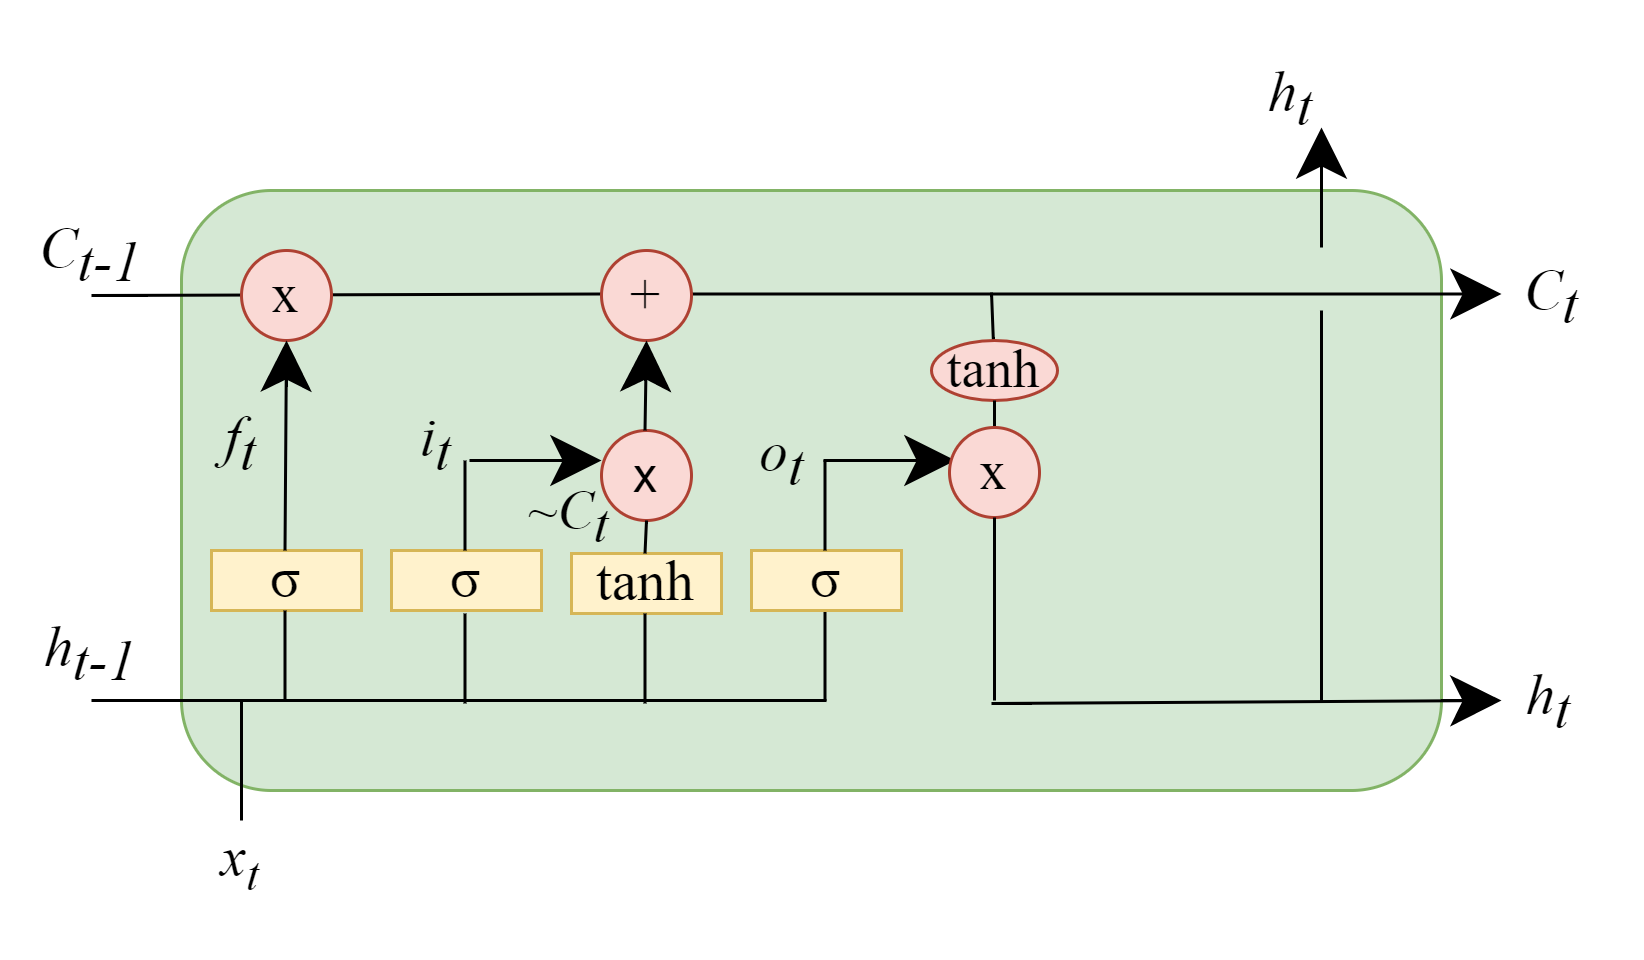
\includegraphics[width=0.9\textwidth]{lstm.png}
\caption{General architecture of LSTM cell.}
\label{lstm}
\end{figure}




\subsubsection{CNN}

In this subsection, we present a brief overview of CNNs. We present the discussion after borrowing the ideas from \cite{singh2020imbalanced}.
CNNs have gained a lot of attention in literature \cite{sinha2022sector}, \cite{miotto2018deep} owing to their ability to address computational issues in a wide variety of applications. The main idea behind a CNN is to take a set of features and filter out the most relevant set of features at every step to make the feature space small. This is usually done with the help of convolutional filters. Generally, there are three major components in a CNN. The first part consists of the input layer. The second category has Convolutional filters that reduce the dimensions by selecting the most relevant set of features. The third part is the pooling layer that the combines output of a set of features. These three subparts work in tandem with each other to find the relevant features as shown in Equation 8. 

\begin{equation}
\varTheta(X) = \varTheta_M (...\Theta_2(\Theta_1(X,\Delta^{(1)}),\Delta^{(2)}),...\Delta^{(Z)})
\end{equation}

where, $\Delta$ is the learning parameter, $M$ represents the total stages, $\Theta$ denote the operations performed at every stage. We  must point out here that the \textit{kernel} plays a major role in the convolutional layer. They produce the necessary feature map. This is fed into the next layer. The following equation 9 represents the process followed here:
\begin{equation}
X_t^{(l)} = \Theta\left(\sum_{i=1}^{M} w_{ji}^{(l)}\ast X_j^{(l-1)}+b_i^{(l)} \right)
\end{equation}

here $\ast$ is called as the convolution operator, $X_i^{(l-1)}$. After this, a nonlinear function, e.g. $ReLU$, is applied to every object. The last part of a CNN is the dense layer, the output of which is passed to the softmax layer for the purposes of classification.

\subsection{Experimentation with Different CNN architecture and Multiple Classification Models}

In the proposed work, the architecture we have followed is presented in Fig. \ref{proposed}. As per this figure, we have used four different convolutional blocks. The dense layer is then fed the output of the convolutional blocks to get the desired result.
We also experimented in this paper by changing the number of convolutional layers.
We specifically change the number of layers from four to three.
We have changed the last dense layer of CNN and introduced SVM as the classification method in addition to changing the number of layers. 
Through numerical investigation, we have found that varying this mode of classification produced the best result.
\begin{figure}
\centering
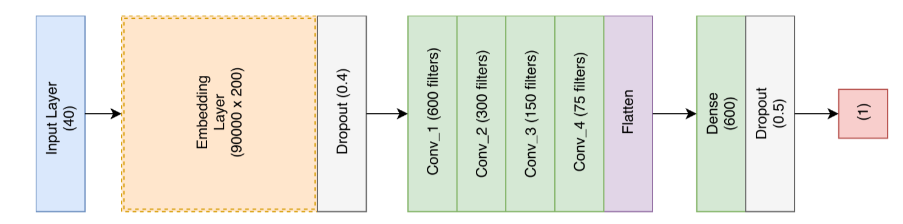
\includegraphics[width=\textwidth]{base.png}
\caption{Proposed architecture of sentiment analysis for Twitter.}
\label{proposed}
\end{figure}


\section{Experimentation Results}
\subsection{Dataset}
The Twitter dataset for sentiment analysis contains tweets and labels indicating the sentiment expressed in the tweet. The dataset consists of tweets along with a sentiment label. The tweets were focused on product reviews. The sentiment labels can be either positive or negative. The dataset, we collected for product reviews, contains more than one Million tweets. Every tweet in the dataset had textual content with the sentiment score associated with the positive and negative classes.

\subsection{Steps Followed in Experimentation}
For the purpose of sentiment classification, the strategy used in the paper is summarized in the following points:
\begin{itemize}
    \item First, the Twitter dataset was pre-processed to remove any special characters. Next, we performed the removal of stop words, stemming, and tokenization of all tweets. 
    \item The dataset consisted of more than 800,000 training tweets. The test dataset had a total of 200,000 tweets.
    \item Next, CNN and LSTM model variations were created. In addition to this, the different variants of CNN as discussed in Section 3.3 were created. 
    \item The data was fed into these models and the performance parameters were computed.
\end{itemize}


\subsection{Ensemble method for sentiment analysis}
To create predictions, ensemble approaches for sentiment analysis combine several models. The details of the proposed ensemble modelling are shown in Figure \ref{hybrid}.

\begin{figure}
    \centering
    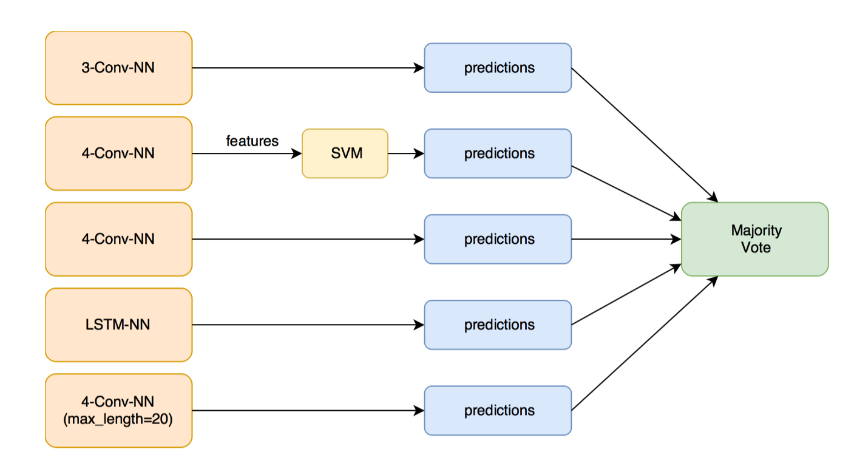
\includegraphics[width=\textwidth]{hybrid.png}
    \caption{Proposed Ensemble approach of Deep Models}
    \label{hybrid}
\end{figure}

We attempted to utilize a vote-based ensemble of the model in this study. The result of the ensemble is shown in Table \ref{tab1}. The ensemble consists of LSTM, CNN with four convolutional layers, CNN with four convolutional layers with SVM as the classification layer, CNN with four convolutional layers with the maximum length of the feature vector as 20, and CNN with three convolutional layers. From the results presented in Table \ref{tab1}, it is clearly visible that the ensemble method and CNN with four convolutional layers with SVM as the classification layer gave the best performance. The reason why the two methods showed the exact same numbers is however unknown. Nevertheless, the method proposed in this article achieved a classification accuracy of 84.95\%. Also, it is observed that the model performs well as the size of the epochs increases. In the experimentation, the model is evaluated on various epoch sizes, whose results are shown in Figure \ref{model-acc}, and found that there is an incremental improvement as the epoch increase. But after the epoch size of 60, the model almost converges with an accuracy of 84.95\%.

\begin{table}[h]
\centering
%\begin{minipage}{140pt}
\caption{Different models and their accuracies.}\label{tab1}%
\begin{tabular}{@{}ll@{}}
\hline
 Model & Accuracy  \\
\hline
LSTM-NN &   83.4\%   \\
4-Conv-NN  &   83.1\% \\
4-Conv-NN-features+SVM &  84.95\%  \\
4-Conv-NN with max-length-20 & 83.85\%   \\
3-Conv-NN       &   83.95\%   \\
 Majority Vote Ensemble  &  84.95\%  \\ 
\hline
\end{tabular}
%\end{minipage}
%\label{tab11}
\end{table}

\begin{figure}
    \centering
    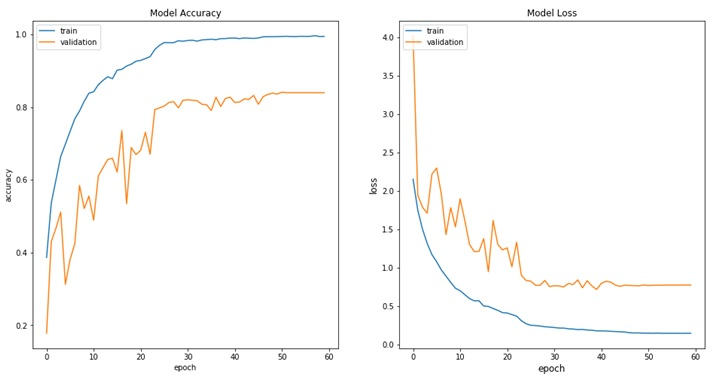
\includegraphics[width=\textwidth]{model-acc.jpg}
    \caption{Performance Evaluation of the proposed model at various epoch sizes}
    \label{model-acc}
\end{figure}

\subsection{Model comparison}

In this subpart, we compare the model's performance with that of related methodologies.
The models under question include namely, bare CNNs, Naive Bayes, MaxEntropy, Decision trees, Random forest, XGBoost, SVM, MLP, LSTM, and the suggested approach. The accuracy statistics are shown in Fig. \ref{accuracyy}. The proposed approach is displaying the best performance, as is seen from the figure. The precise number for accuracy is 84.95\%. This outcome unequivocally demonstrates the method's superiority over some of the current machine learning models. 


\begin{figure}[t]
\centering
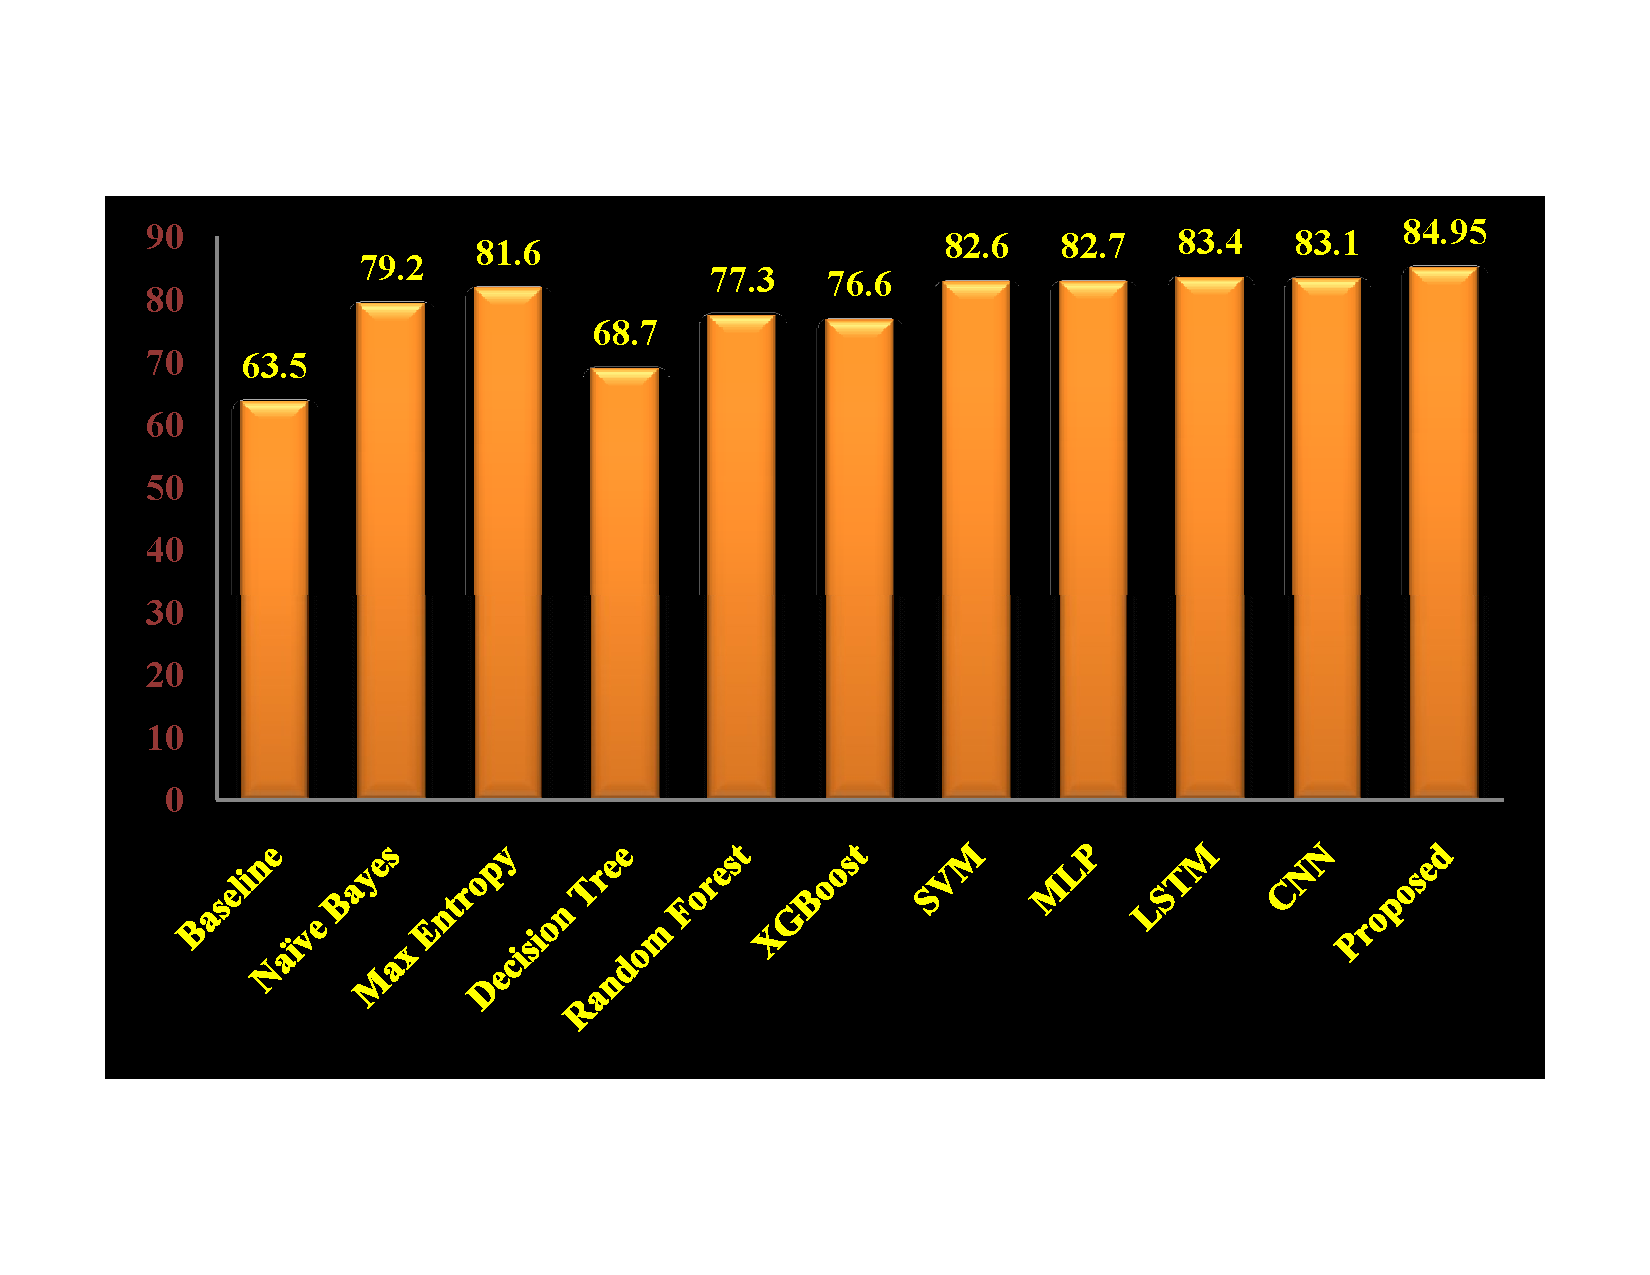
\includegraphics[width=0.9\textwidth]{res.pdf}
\caption{Different model comparison of sentiment analysis for Twitter.}
\label{accuracyy}
\end{figure}

\section{Discussion}

In this section, we discuss the shortcomings of the proposed work. 
\begin{itemize}
\item A disadvantage of sentiment analysis of Twitter for classification using a convolutional neural network is that the data is not always precise. For example, a tweet that is generally positive could be labeled wrongly. Additionally, the sentiment of a tweet may change over time, so it may not be accurate to label a tweet as positive or negative based on its sentiment when it was initially posted.

\item The next issue is data accessibility.
Twitter data is frequently loud and unstructured, which makes it challenging to train the neural network.
Typos and abbreviations make it more challenging to understand the emotion and meaning of a tweet.
Additionally, there are instances in which a Tweet's language may be bilingual or multilingual.
Therefore, we do not address the issue of automatic sentiment categorization of Tweets in this paper. 

\item Optimization of hyperparameters is the subsequent issue. It is a well-accepted fact that a neural network depends on several hyperparameters. In this article, we used brute force to identify the ideal set of parameters. We will need to develop automated methods in the future to select the proper set of parameters. 
\end{itemize}


\section{Conclusion and Future Work}

One of the most promising areas of computational analysis is sentiment categorization.
In this study, we suggested a novel approach to categorizing sentiments. The concept of N-gram-based word embeddings was employed to generate the vector representation of tweets from Twitter.
The categorization of tweets as favorable or unfavorable was then carried out using automated machine-driven procedures. For this purpose, experiments were conducted via LSTM and different variants of CNN. Further, the last layer of CNN was modified and multiple classification modes were tried. Lastly, the methods were combined using an ensemble scheme of classification. It was found that the ensemble approach of the various CNN models increases the accuracy of the system. One of the reasons for this positive model feedback is the hybridization of the different feature pool sizes using various CNN models. Each of the models is utilized to fetch the different feature pools using the N-gram approach. This collective information may be providing a better intuition of the results. Further, the testing of the method was performed on the Twitter Dataset consisting of more than One Million Tweets. Extensive numerical investigation revealed the superior performance of the proposed technique. Comparison with other existing Machine learning methods also indicated that the work presented in the article shows promise in terms of practical deployment. In this article, we experimented with N-gram-based word embedding. In the future, we would be experimenting with BERT-based embeddings. 

% \section*{Compliance with Ethical Standards}
% \subsection*{Conflict of Interest:}
% The authors of this manuscript declare that there is no conflict of interest.

% \subsection*{Funding Information:}
% The author declares that there is no funding associated with this project. 

% \subsection*{Ethics Statement:}
% The author of this manuscript confirms that:
% (i)  Informed, written consent has been obtained from the relevant sources wherever required;
% (ii) All procedures followed were in accordance with the ethical standards of the responsible committee on human experimentation (institutional and national) and with the Helsinki Declaration of 1964 and its later amendments.


%\bibliographystyle{spmpsci}
\bibliographystyle{elsarticle-num} 
\bibliography{sn-bibliography}% common bib file
%% if required, the content of .bbl file can be included here once bbl is generated
%%\input sn-article.bbl

%% Default %%
%%\input sn-sample-bib.tex%

\end{document}
